%% Congresso Brasileiro de Fisica Medica (CBFM)
%% 
%% Nome: Rodrigo de Barros Vimieiro
%% Nome: Vinícius Paranaíba Campos
%% 
%%
%% Universidade de São Paulo - São Carlos
%% Laboratório de Visão Computacional - LAVI
%%
%% Data: 10/04/2019

% vvvvvvvvvvvvvvvvvvvvv
% Compiled with XeLateX
% ^^^^^^^^^^^^^^^^^^^^^

\documentclass[10pt,twoside,twocolumn]{article}
\bibliographystyle{vancouver}

%%%%%%%%%%%%%%%%%%%% Packages %%%%%%%%%%%%%%%%%%%%

\usepackage[utf8]{inputenc}
\usepackage{fontspec}
\setmainfont{Arial}
\usepackage{fancyhdr}
\renewcommand{\footrulewidth}{0.4pt}
\usepackage[]{caption}
\captionsetup[figure]{labelsep = endash,skip=-10pt,font=small,labelfont=bf}
\captionsetup[table]{labelsep = endash,skip=0pt,font=small,labelfont=bf}
\usepackage{titlesec}
\titleformat*{\section}{\normalsize\bfseries}
\titleformat*{\subsection}{\normalsize\itshape}
\titlelabel{\thetitle.\quad}
\titlespacing*{\section}{0pt}{10pt}{3pt}
\titlespacing*{\subsection}{0pt}{10pt}{3pt}
\usepackage{graphicx}
\usepackage{amsmath}
\usepackage{hyperref}
\hypersetup{
    	colorlinks=true, % false: boxed links; true: colored links
        linkcolor=black,          	% color of internal links
        urlcolor=blue,
        citecolor=black
}
\usepackage{indentfirst}
\usepackage{amssymb}
\usepackage{lipsum}
\usepackage{xcolor}
\usepackage{etoolbox}
\AtBeginEnvironment{thebibliography}{\interlinepenalty=10000}
\usepackage{geometry}
 \geometry{
 a4paper,
 top = 1.5cm,
 headsep=10pt,
 width=17.2cm,
 inner=2cm,
 outer=1.8cm,
 }
\usepackage[super]{natbib} 
\makeatletter
\renewcommand*{\@biblabel}[1]{\hfill#1.}
\makeatother
 
 %%%%%%%%%%%%%%%%%%%% Color notations %%%%%%%%%%%%%%%%%%%%
 
 \newcommand{\rv}[1]{{\textcolor[rgb]{.5,.7,.15}{\small[\textbf{Rodrigo}: #1]}}}	%(Rodrigo)
\newcommand{\lb}[1]{{\textcolor[rgb]{.5,.0,.0}{\small[\textbf{Lucas}: #1]}}}	%(Lucas)
\newcommand{\RV}[2]{{\textcolor[rgb]{.5,.7,.15}{\uwave{#1 }\small[\sout{#2}]}}} %(Rodrigo)
\newcommand{\LB}[2]{{\textcolor[rgb]{.5,.0,.0}{\uwave{#1 }\small[\sout{#2}]}}} %(Lucas)
\newcommand{\rb}[1]{{\textcolor[rgb]{.1,.1,.5}{\small[\textbf{Renann}: #1]}}}	%(Renann)
 
 
 %%%%%%%%%%%%%%%%%%%% Begin document %%%%%%%%%%%%%%%%%%%%
 
\begin{document}


%%%%%%%%%%%% Headers and footers %%%%%%%%%%%% 

\pagestyle{fancy}
\fancyhf{}
\fancyfoot{}
\lhead{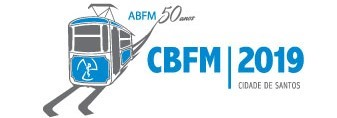
\includegraphics[height=1.8cm]{heads/CBFM_head.jpg}}
\rhead{
        \large \textbf{XXIV Congresso Brasileiro de Física Médica\\
        21 a 24 de Agosto de 2019\\
        Santos}
}
\rfoot{\small \thepage}
\lfoot{\small \textit{Associação Brasileira de Física Médica}\space \textregistered}

%%%%%%%%%%%%%%%%%%%%%%%%%%%%%%%%%%%%%%%%%%%%%%%%%%%%%%%%%%%%%%%%%%%%%%%%%
%                                                                       %
%%%%%%%%%%%%%%%%%%%%%%%%%%%%%%%%%%%%%%%%%%%%%%%%%%%%%%%%%%%%%%%%%%%%%%%%%

%%%%%%%%%%%% Headers informations %%%%%%%%%%%%

\twocolumn[\vspace{40pt}
  \begin{@twocolumnfalse}
  
    \begin{flushright}

        \Large{
        \textbf{Assessment of dose reduction simulation in digital breast tomosynthesis system with amorphous silicon (a-Si) detector}
        }
        
        \Large{
        Information for Authors for Full Paper Submission\\
        to the Congresso Brasileiro de F\'{i}sica M\'{e}dica
        }
        
        \vspace{\baselineskip}
        
        \large{
        Primeiro A. Autor$^{1}$, Segundo B. Co-autor$^{2}$, \'{U}ltimo C. Co-autor$^{3}$\\
        }
        
       \vspace{\baselineskip}
       
       \normalsize{
        
        $^{1}$\textit{Institui\c{c}\~{a}o/Afilia\c{c}\~{a}o, Cidade, Pa\'{i}s}
        
        $^{2}$\textit{Divis\~{a}o/Servi\c{c}o/Departamento, Instituto/Hospital/Universidade, Cidade, Pa\'{i}s}
        
        $^{3}$\textit{Servi\c{c}o/Departamento, Hospital/Universidade, Cidade, Pa\'{i}s}
        
        }

    \end{flushright}

%%%%%%%%%%%%%%%%%%%%%%%%%%%%%%%%%%%%%%%%%%%%%%%%%%%%%%%%%%%%%%%%%%%%%%%%%
%                                                                       %
%%%%%%%%%%%%%%%%%%%%%%%%%%%%%%%%%%%%%%%%%%%%%%%%%%%%%%%%%%%%%%%%%%%%%%%%%

%%%%%%%%%%%% Resumo %%%%%%%%%%%%

\noindent\rule{17.2cm}{0.4pt}
\textbf{Resumo}

Este modelo apresenta as instruções para a submissão de artigos completos ao Congresso Brasileiro de Física Médica (CBFM). Os artigos devem ser submetidos eletronicamente pelo website da CBFM. Serão aceitos artigos em português, espanhol e inglês, com, no mínimo, 4 (quatro) páginas, e no máximo, 10 (dez) páginas. O resumo/abstract deve conter, no mínimo 150 e no máximo, 300 palavras. Sempre que o artigo for escrito em língua estrangeira, um resumo em português é exigido. Devem ser listados, abaixo do resumo, de 3 (três) até 6 (seis) unitermos/palavras-chave, preferencialmente de acordo com os Descritores em Ciências da Saúde (DeCS) ou com o Medical Subject Headings (MeSH) da National Library of Medicine (http://www.nlm.nih.gov), ou com o Physics and Astronomy Classification Scheme (PACS - http://www.aip.org/pacs/index.html), separados por ponto e vírgula. As referências devem ser numeradas e citadas de acordo com a ordem de aparecimento no artigo. As referências devem ser escritas ao estilo Vancouver.

\textbf{Palavras-chave}: f\'{i}sica m\'{e}dica; medicina nuclear; radioterapia; radiologia; prote\c{c}\~{a}o radiol\'{o}gica.\\


%%%%%%%%%%%% Abstract %%%%%%%%%%%%

\textbf{\textit{Abstract}}

\textit{This model presents the instructions for submitting full papers to the Brazilian Congress of Medical Physics (CBFM). The papers must be submitted electronically in CBFM website. Papers will be accepted in Portuguese, Spanish and English, with a minimum of 4 (four) pages and a maximum of 10 (ten) pages. The abstract should contain a minimum of 150 and a maximum of 300 words. Whenever the article is written in a foreign language, a summary in Portuguese is mandatory. Three (3) to six (6) keywords should be listed below the abstracts, preferably in accordance with the Health Sciences Descriptors (DeCS) or the Medical Subject Headings (MeSH) of the National Library of Medicine (http://www.nlm.nih.gov), or the Physics and Astronomy Classification Scheme (PACS - http://www.aip.org/pacs/index.html), separated by a semicolon. References should be numbered and quoted according to the order of appearance in the article. The references must de written in the Vancouver style.}

\textbf{Keywords}\textit{: medical physics; nuclear medicine; radiation oncology; radiology; radiation protection.} 
\noindent\rule{17.2cm}{0.4pt}
\vspace{\baselineskip}
    \end{@twocolumnfalse}
 ]
 
%%%%%%%%%%%%%%%%%%%%%%%%%%%%%%%%%%%%%%%%%%%%%%%%%%%%%%%%%%%%%%%%%%%%%%%%%
%                                                                       %
%%%%%%%%%%%%%%%%%%%%%%%%%%%%%%%%%%%%%%%%%%%%%%%%%%%%%%%%%%%%%%%%%%%%%%%%%
 
%%%%%%%%%%%% Introduction %%%%%%%%%%%% 
 
\section{Introduction}

\lipsum

\section{Theoretical Background}
\subsection{Background}

\lipsum

\subsection{Noise model}


\lipsum

\begin{equation}
\label{eq.Eq2}
 \sigma(y(i,j)) = \sqrt{\lambda(i,j) \, y(i,j) + \sigma^{2}_{e}},
\end{equation}


\section{Materials \& Methods}

\lipsum


\begin{table}[ht]
\caption{DBT system characteristics \cite{vedantham2015digital}.}
	\label{tab:tab1}
   	\centering
% 	\footnotesize
	\begin{tabular}{l|c}
		\textbf{Characteristic}                                       &        \textbf{}              \\
		[1pt]
		\hline
        \rule[-0.5ex]{-3pt}{1ex}
		Detector type                 &         CsI:Tl (Indirect)                               \\ \hline
       	\rule[-0.5ex]{-3pt}{1ex}
		Manufacturer &    General Electric    \\ \hline
		\rule[-0.5ex]{-3pt}{1ex}
		Model &    Senographe Essential    \\ \hline
		\rule[-0.5ex]{-3pt}{1ex}
		Projection number              &                9                                               \\ \hline
		\rule[-0.5ex]{-3pt}{1ex}
		Tube angle span                &           $25^{\circ}$          		                          \\ \hline
		\rule[-0.5ex]{-3pt}{1ex}
		Detector angle span           &          Stationary                                  \\ \hline
		\rule[-0.5ex]{-3pt}{1ex}
		Tube movement                &     Step-and-shoot                              \\ \hline
		\rule[-0.5ex]{-3pt}{1ex}
		Pixel size        &            100$\mu$m                                \\ \hline
	\end{tabular}
	\caption*{Fonte: O autor(2019).}
\end{table}

\section{Results \& Discussion}

\lipsum

\begin{figure}[!ht]
    \caption{Modelo.}
    \label{fig:img1}
	\begin{center}
		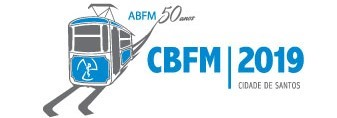
\includegraphics[scale=.56]{heads/CBFM_head.jpg}
	\end{center}
	\caption*{Fonte: O autor(2019).}
\end{figure}




\section{Conclusion}

\lipsum

\section*{Acknowledgments}

\lipsum

\small{
\bibliography{bibliography}
}

\end{document}

